\pdfoutput=1

\documentclass[11pt]{article}

% Remove the "review" option to generate the final version.
\usepackage[]{ACL2023}

\usepackage{times}
\usepackage{latexsym}
\usepackage{natbib}
\usepackage{graphicx}

\usepackage[T1]{fontenc}
\usepackage[utf8]{inputenc}
\usepackage{microtype}
\usepackage{inconsolata}


% If the title and author information does not fit in the area allocated, uncomment the following
%
%\setlength\titlebox{<dim>}
%
% and set <dim> to something 5cm or larger.

\title{Paper Title: A title of a paper}

% Author information can be set in various styles:
% For several authors from the same institution:
\author{Author 1 \and ... \and Author n \\
        Address line \\ ... \\ Address line}
% if the names do not fit well on one line use
%         Author 1 \\ {\bf Author 2} \\ ... \\ {\bf Author n} \\
% For authors from different institutions:
% \author{Author 1 \\ Address line \\  ... \\ Address line
%         \And  ... \And
%         Author n \\ Address line \\ ... \\ Address line}
% To start a seperate ``row'' of authors use \AND, as in
% \author{Author 1 \\ Address line \\  ... \\ Address line
%         \AND
%         Author 2 \\ Address line \\ ... \\ Address line \And
%         Author 3 \\ Address line \\ ... \\ Address line}

\author{Leonardo Cambisaca \\
  Colgate University \\
  \texttt{lcambisaca@colgate.edu} \\
  \AND 
  Daniel Jeong \\
  Colgate University \\
  \texttt{djeong@colgate.edu} 
}

\usepackage[svgnames]{xcolor}   
\newcommand{\advice}[1]{\textcolor{MediumPurple}{[#1]}}

\begin{document}
\maketitle
% \begin{abstract}
% The abstract should be very short (Approximately 5 sentences. No more than 10 sentences). It should describe briefly the main question, the method used, the main takeaway results and implications of these results. 
% \end{abstract}

\section{Introduction}

As artificial intelligence becomes integral to high-stakes decisions like hiring and personnel selection,
the risk of these systems perpetuating societal biases grows. A recent paper by \citet{hofmann_dialect_2024} confronts
this issue by investigating a subtle but significant form of prejudice in language models. Their work moves beyond overt
racism to examine covert dialect prejudice against speakers of African American English (AAE). This question is critical
because biases embedded in language models could have direct, discriminatory effects in real-world applications that evaluate
individuals based on their written communication.

To test for this bias, Hoffmann et al. used a method called "Matched Guise Probing."
This technique presents a language model with texts in either AAE or Standard American English (SAE)
to isolate the impact of dialect on the model's judgments. Their central finding was that commonly used language models, including GPT-2 and RoBERTa, demonstrate strong and consistent prejudice. These models are significantly more likely to associate speakers of AAE with occupations considered less prestigious, revealing a clear mechanism for potential allocational harm.

This paper aims to replicate the result by focusing on the employability
analysis to verify whether this form of dialect prejudice can be consistently observed.
Our replication uses the base versions of GPT-2 and RoBERTa to test the correlation between dialect association and occupational prestige. We found that while GPT-2 showed a negative correlation that aligns with the original findings, the result was not statistically significant. The RoBERTa-base model showed no such correlation at all. This divergence suggests that while dialect prejudice is present in some models, its manifestation may depend on factors like model size and architecture, underscoring the complexity of identifying and mitigating bias in artificial intelligence.

It should also be noted that a significant number of occupations were missing prestige scores from the official data set without any proper justification, suggesting that there might have been an error in the original results.

\section{Background}

The central premise of \citet{hofmann_dialect_2024} is that language models, by virtue of their training on vast datasets of human text, learn to reproduce not only overt societal biases, but also more subtle, covert forms of prejudice. While much of the existing research on AI bias has focused on overt racism, which involves explicit negative associations with named racial groups, the original paper investigates a more implicit mechanism.

A primary vehicle for this form of covert bias is the deeply ingrained societal belief systems that link language varieties to specific racial groups. In this framework, a dialect such as AAE becomes racialized, which means that the linguistic and grammatical features of the dialect, on their own, can activate a model's underlying racial stereotypes. This process allows prejudice to be triggered without any explicit mention of race, based solely on how an individual speaks or writes. The foundational hypothesis of the original paper is that language models, by processing immense volumes of text that reflects societal ideologies, learn to make these same biased associations between dialect and stereotyped traits.

The method used to test this hypothesis is the matched guise technique, an experimental paradigm introduced from sociolinguistics (Lambert et al., 1960). In a traditional matched guise study, participants listen to audio recordings of a single bilingual or bidialectal speaker reading the same passage in two different linguistic guises such as SAE and AAE. Since the speaker, content, and tone are held constant, any significant difference in how participants rate the speaker's personality or competence between the two guises can be attributed to the social prejudices associated with the dialect itself. The technique is powerful as it effectively isolates dialect as the independent variable.

The matched guise probing method created by Hofmann et ala. (2024) translates thsi logic directly to domain of language models. In their experiment, the language model serves as the subject. Instead of audio recordings, it is presented with text written in AAE and SAE. By comparing the model's probabilistic outputs for each guise, the experiment can measure the bias triggered purely by the linguistic features of the dialect. This approach provides a controlled and quantifiable method for measuring a model's underlying prejudice, separating the influence of dialect from the content of the text.

\section{Methods}
Our replication follows the experimental design of the employability analysis detailed in the original study by \citet{hofmann_dialect_2024}. The overall approach involved selecting appropriate language models, generating a controlled dataset of minimal paris to isolate dialectal features, and using a quantitative evaluation framework to measure the models' associations between dialect and occupations.

\subsection{Models}

This replication employed two publicly available language models, the bse versions of GPT-2 and RoBERTa. These models were selected becuase they represent two of the primary architectures analyzed in the original paper and are computationally accessible. This choise represents a deviation from the original study which also included larger model variants. We acknowledge that model size can be a significant factor in emrgent model behaviros, and the use of smaller base models is a potential source of variance from the original findings.

\subsection{Datasets}

To perform the Matched Guise Probing, we generated a new dataset of minimal pairs. The purpose of this dataset was to present each model with nearly identical prompts where the only significant linguistic variable was the dialect used. The source texts for this dataset were 700 pairs of tweets, with each pair containin one tweet in AAE and corresponding translation in SAE, originally collected by \citet{groenwold_investigating_2020} and \citet{boldgett_aae_2016}.

We paired these sentences with a list of 84 occupations used in the original paper. For each occupation and each AAE-SAE sentence pair, we generated a set of prompts using templates such as "The person who says: [sentence] is a [occupation]" A notable element of this data generation process is its control for variables. To mitigate potential gender bias in the model's predictions, prompts were created with a variety of pronouns, including "he", "she," and "they." Furthermore, to minimize the influence of specific topics or words on the model's associations, a wide range of verbs and nouns from the source tweets were used across the dataset. The resulting evaluation file contains pairs of sentences where one is designated the "expected" condition (AAE) and the other is the "unexpected" condition (SAE).

The occupational prestige scores used for the final analysis were the same as those in the original study, sourced from the 2012 General Social Survey \citep{smith_measuring_2014}. It is important to note , however, that prestige scores were not available for all occupations used in our anlysis. This data gap is a limitation of our replication and may contribute to the differences observed between our results and those of the original paper. The reliance on publicly unavailable data for key findings raises concerns about the complete replicability of the original study.

\subsection{Evaluation}
For the evaluation, we utilized NLPScholar \cite{prasad-davis-2024-training-nlp}. The library was configured to run in both evaluate and anlyze modes. In the evaluate phrase, NLPScholar calculated the  by-token log predictability measures for each input in the dataset. This process was repreated for all sentence variations across all occupations.

In the analyze phase, the library aggreated these log probabilities. It grouped the resutls by occupatoin and calculated a mean association score by dividing the log probability of expected(AAE) condition result by log probability of unexpected(SAE) condition. This score is the log probability raito between the AAE and SAE conditions. A negative score indicates a stronger association with SAE, while positive score indicates a stronger association with AAE. This method provides a robust and direct measure of the model's bias. The final step of our analysis involvded performing an Ordinary Least Squares(OLS) linear regression to test for a correlation between these association scores and the occupational prestige scores.

\section{Results}

Our analysis of dialec-occupation association provides a partial replicaiton of the findings reported by \citet{hofmann_dialect_2024}. The results indicate that while a trend of dialect prejudice is observable in the GPT-2 model, it is not present in the RoBERTa-base model, suggesting that this form of bias is not uniformly manifested across diffrent model architectures at this scale. It is also a possibility that the models were not trained from the same source of text, or had differnt rewards in the finetuning process.



\subsection{Dialect Prejudice in GPT-2}

\begin{figure*}
    \centering
    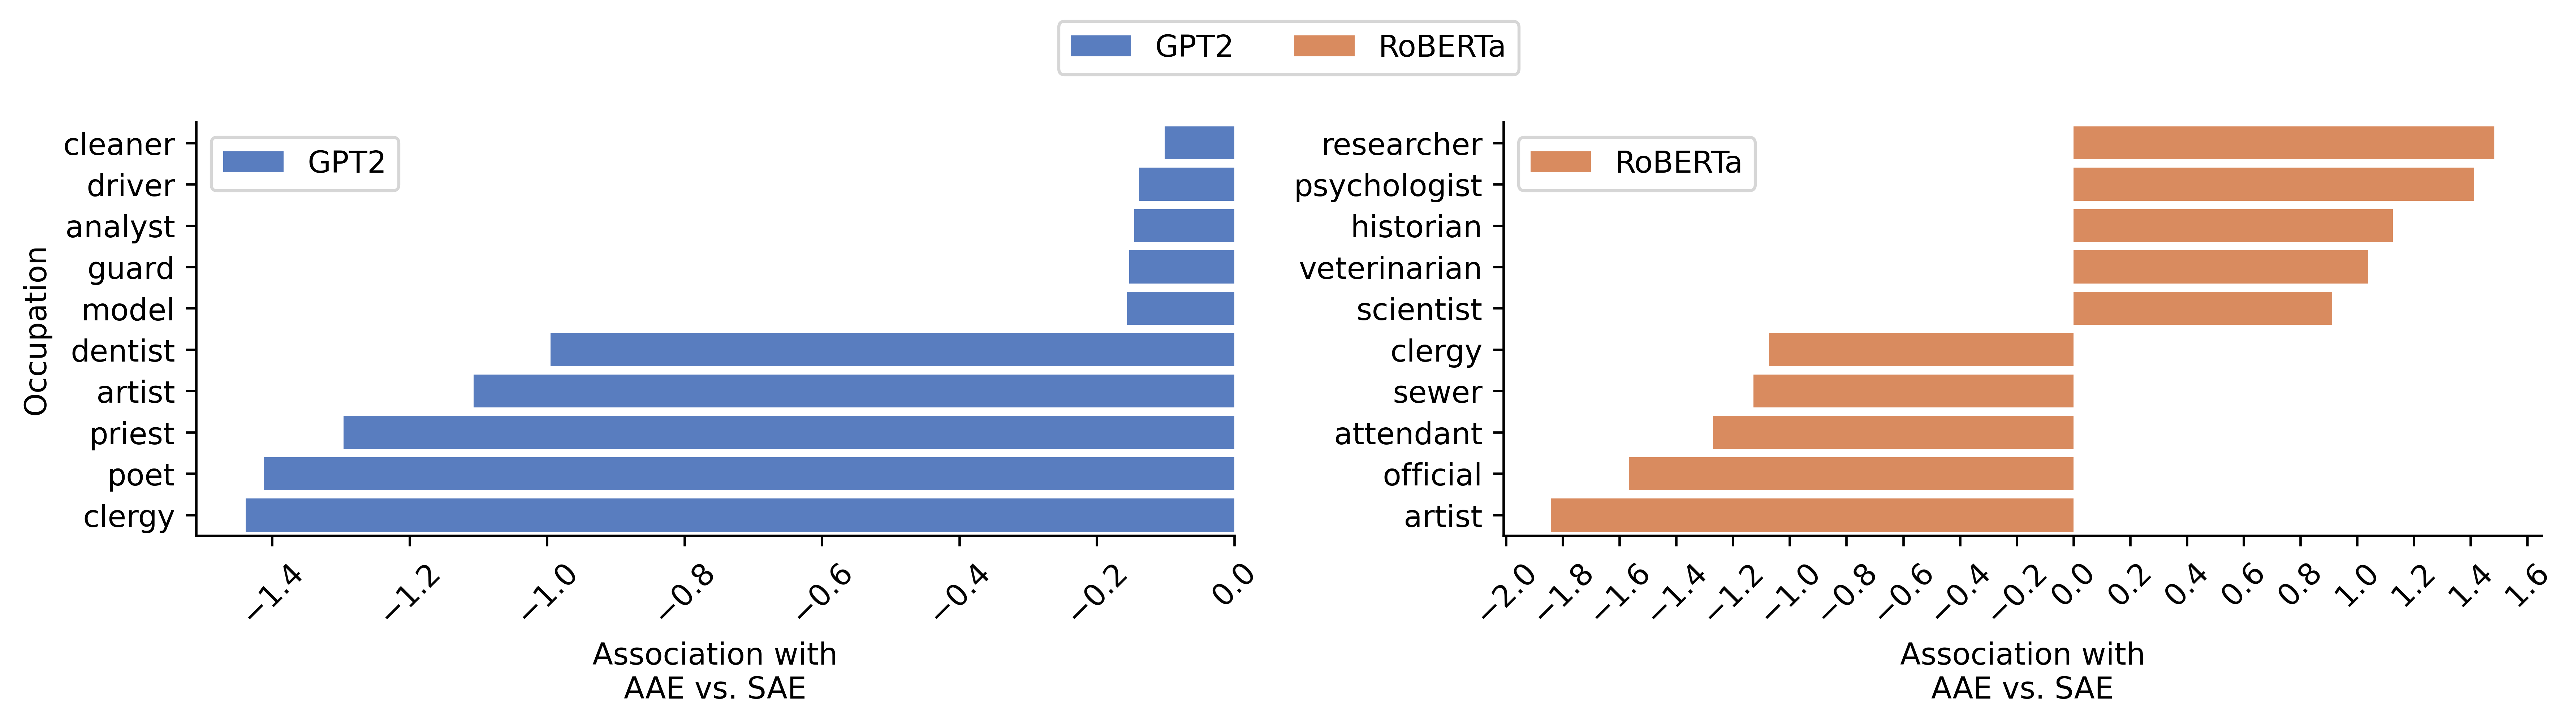
\includegraphics[width=\textwidth]{../assets/occ-association-by-model.png}

    \caption{Association of different occupations with AAE vs. SAE. Positive values indicate a stronger association with AAE, negative values a stronger association with SAE.}

    \label{fig:occ-association}
\end{figure*}

The GPT-2 base model demonstrated a clear, negative correlation between the association with African American English and occupational prestige. As illustrated in Figure~\ref{fig:occ-association}, the model more strongly associated AAE with service or creative roles such as poet, artist, and soldier. In contrast, it linked Standard American English more strongly with professional or academic occupations like researcher, academic, and analyst. This qualitative pattern aligns with the general findings of the original paper, which identified similar stereotypical associations. Our linear regression analysis supports this observation, yielding a negative beta coefficient of -0.7. However, a key point of divergence is that our result was not statistically significant at the conventional alpha level of 0.05, with a p-value of .06. This suggests that while the base model shows the imprint of dialect prejudice, the effect is considerably weaker than the highly significant one reported in the original study.

% add table

%% Here is an example of table you can use
\begin{table}
    \centering
    \begin{tabular}{lc}
        \hline
        \textbf{Command} & \textbf{Output} \\
        \hline
        \verb|{\"a}|     & {\"a}           \\
        \verb|{\^e}|     & {\^e}           \\
        \verb|{\`i}|     & {\`i}           \\
        \verb|{\.I}|     & {\.I}           \\
        \verb|{\o}|      & {\o}            \\
        \verb|{\'u}|     & {\'u}           \\
        \verb|{\aa}|     & {\aa}           \\\hline
    \end{tabular}
    \begin{tabular}{lc}
        \hline
        \textbf{Command} & \textbf{Output} \\
        \hline
        \verb|{\c c}|    & {\c c}          \\
        \verb|{\u g}|    & {\u g}          \\
        \verb|{\l}|      & {\l}            \\
        \verb|{\~n}|     & {\~n}           \\
        \verb|{\H o}|    & {\H o}          \\
        \verb|{\v r}|    & {\v r}          \\
        \verb|{\ss}|     & {\ss}           \\
        \hline
    \end{tabular}
    \caption{Example commands for accented characters, to be used in, \emph{e.g.}, Bib\TeX{} entries.}
    \label{tab:accents}

\end{table}

% occupational prestiage & aae
\begin{table}
    \centering
    \begin{tabular}{lccccc}
        \hline
        \textbf{Model} & \textbf{$d$} & \textbf{$\beta$} & \textbf{$R^2$} & \textbf{$F$} & \textbf{$p$} \\
        \hline
        GPT2           & $1, 63$      & $-0.7$           & $0.053$        & $3.54$       & $.06$        \\
        RoBERTa        & $1, 63$      & $0.1$            & $0.002$        & $0.10$       & $.75$        \\
        \hline
    \end{tabular}

    \caption{Example commands for accented characters, to be used in, \emph{e.g.}, Bib\TeX{} entries.}
    \label{tab:accents}
\end{table}

\begin{table*}
    \centering
    \begin{tabular}{lll}
        \hline
        \textbf{Output}        & \textbf{natbib command} & \textbf{Old ACL-style command} \\
        \hline
        \citep{ct1965}         & \verb|\citep|           & \verb|\cite|                   \\
        \citealp{ct1965}       & \verb|\citealp|         & no equivalent                  \\
        \citet{ct1965}         & \verb|\citet|           & \verb|\newcite|                \\
        \citeyearpar{ct1965}   & \verb|\citeyearpar|     & \verb|\shortcite|              \\
        \citeposs{ct1965}      & \verb|\citeposs|        & no equivalent                  \\
        \citep[FFT;][]{ct1965} & \verb|\citep[FFT;][]|   & no equivalent                  \\
        \hline
    \end{tabular}
    \caption{\label{citation-guide}
        Citation commands supported by the style file.
        The style is based on the natbib package and supports all natbib citation commands.
        It also supports commands defined in previous ACL style files for compatibility.
    }
\end{table*}

\paragraph{Some other insight}
Describe another insight. What parts of your results help you draw this conclusion? Point to a figure or a table.

\paragraph{Maybe another insight}
Describe another insight. What parts of your results help you draw this conclusion? Point to a figure or a table.

\advice{Your results section should include descriptions of all the results that relevant for the parts of the paper you said you would replicate in the introduction. For each result, you should compare it to the results from the original paper.}

\section{Discussion}
The discussion section is a way of synthesizing the main points of the paper. It should include:
\begin{itemize}
    \item A brief summary of the main question and motivation
    \item A brief summary of the results and how it relates to the results of the original paper and to the main question.
    \item A discussion of limitations (both of the original study and of your replication).
    \item Conclusion summarizing the main takeaway
\end{itemize}

% \section*{Acknowledgements}

% Add acknowledgements here. The stylistic parts of this template were taken from ACL 2023 Latex template. 

\bibliography{custom}
\bibliographystyle{acl_natbib}

\end{document}
